\documentclass[12pt]{report}
\usepackage[utf8]{inputenc}
\usepackage{amsmath}
\usepackage{graphicx}
\usepackage{bm}
\usepackage{xcolor}
\usepackage{listings}
\usepackage{hyperref}
\usepackage{natbib}
\usepackage{booktabs}

\lstset{
  language=Python,
  basicstyle=\ttfamily\small,
  columns=fullflexible,
  breaklines=true,
  keywordstyle=\color{blue},
  commentstyle=\color{gray},
  stringstyle=\color{teal},
  frame=single,
  numbers=left,
  numberstyle=\tiny,
  stepnumber=1
}

\title{\bfseries%
Project 2: Tree predictors for binary classification\\[4pt]
\large + Random Forest}
\author{Marcello Calza}
\date{31 May 2025}

\begin{document}
\maketitle
\tableofcontents
\clearpage

\emph{I/We declare that this material, which I/We now submit for assessment, is entirely my/our 
own work and has not been taken from the work of others, save and to the extent that such 
work has been cited and acknowledged within the text of my/our work. I/We understand that 
plagiarism, collusion, and copying are grave and serious offences in the university and 
accept the penalties that would be imposed should I engage in plagiarism, collusion or 
copying. This assignment, or any part of it, has not been previously submitted by me/us 
or any other person for assessment on this or any other course of study.}

\section{Introduction}

The project implements, from scratch, a full predictive pipeline able to decide whether
a mushroom is \textit{poisonous} or \textit{edible}. The workflow consists of

\begin{enumerate}
  \item data wrangling and encoding of categorical attributes;
  \item greedy decision-tree induction with three impurity measures;
  \item random forest ensemble;
  \item single-level 10-fold cross-validation (CV) for hyper-parameter tuning;
  \item bias-variance diagnostics via empirical proxies.
\end{enumerate}

The code is organised in five lean modules: \texttt{criteria.py}, \texttt{tree.py},
\texttt{forest.py}, \texttt{tuning.py}, \texttt{diagnostics.py} - plus a 200-line driver
script \texttt{run.py}.  Each section below integrates

\begin{itemize}
  \item theoretical background,
  \item implementation highlights,
  \item experimental evidence.
\end{itemize}

\section{Tree predictor}

\subsection{Theory and design}
The predictor follows the recursive strategy of \citet[pp.\,253-254]{shalev}.\
Starting from a single leaf predicting the majority label, the algorithm repeatedly
replaces the leaf that yields the \emph{largest impurity decrease}
\[
  \Delta\psi
  =\psi(S)
  -\frac{|S_L|}{|S|}\psi(S_L)
  -\frac{|S_R|}{|S|}\psi(S_R).
\]

Here  

\begin{itemize}
  \item \(S\) is the multiset of training pairs reaching the current leaf;
  \item \(S_L=\{(x,y)\!\in\!S : x_i=1\}\) and
        \(S_R=\{(x,y)\!\in\!S : x_i=0\}\) are the left/right children
        produced by the candidate split on feature~\(i\);
  \item \(\psi(\cdot)\) is any impurity surrogate
        (Gini, scaled entropy, square-root).
\end{itemize}

Three concave surrogates are implemented and selectable as the impurity criterion:
\begin{itemize}
  \item $\psi_2$: Gini impurity, $2p(1-p)$;
  \item $\psi_3$: half-scaled Shannon entropy, $-\tfrac{1}{2}[p \log_2 p + (1-p)\log_2(1-p)]$;
  \item $\psi_4$: square-root impurity, $\sqrt{p(1-p)}$.
\end{itemize}

These were recommended in the lectures because they avoid the flat regions of
$\min\{p,1-p\}$.

Real-valued features are split by enumerating mid-points between consecutive sorted
values \citep[p.\,255]{shalev}.  Early stopping controls the capacity:

\begin{itemize}
  \item maximum depth $d_{\max}$;
  \item minimum samples per leaf $m_{\text{leaf}}$;
  \item minimum impurity decrease $\epsilon$.
\end{itemize}

\subsection{tree.py module}
\texttt{tree.py} contains the main building blocks for decision-tree induction:

\begin{description}
  \item[\texttt{Node}]
        Represents a single node in the tree, which can be either an internal split or
        a leaf prediction.
    \begin{description}
      \item[\texttt{\_\_init\_\_}]
            Initializes the node as a split (with a decision rule) or as a leaf (with a
            class prediction).
      \item[\texttt{\_\_call\_\_}]
            Applies the node's split rule to a batch of samples, returning which
            samples go left (if split node) or does nothing (if leaf).
    \end{description}

  \item[\texttt{DecisionTree}]
        Constructs and manages a binary classification tree using greedy impurity
        minimization and several stopping conditions.
    \begin{description}
      \item[\texttt{\_\_init\_\_}]
            Sets up the impurity criterion, stopping parameters, and feature handling.
      \item[\texttt{fit}]
            Builds the tree recursively from the training data, splitting nodes based
            on impurity reduction until stopping.
      \item[\texttt{predict}]
            Assigns class labels to new samples by traversing the fitted tree from root
            to leaf.
      \item[\texttt{\_grow}]
            Recursively constructs each subtree, picking the best split at each node
            according to impurity gain and creating leaves when needed.
      \item[\texttt{\_infer}]
            Follows the decision path for a single sample to retrieve its predicted
            label.
      \item[\texttt{\_majority}]
            Finds the most frequent label in a set (used for majority vote at leaves).
    \end{description}
\end{description}

Key points inside \texttt{DecisionTree}:

\begin{itemize}
  \item column-wise caching of unique categories removes redundant
        \texttt{np.unique} calls in deep sub-trees;
  \item recursion passes \textbf{index masks} instead of slicing the whole
        feature matrix; avoids $O(n\log n)$ copying;
  \item optional \texttt{max\_features} parameter so the same class can be used
        by the random forest.
\end{itemize}

\subsection{Results}
10-fold CV selected $\psi_3$, $d_{\max}=25$, $m_{\text{leaf}}=10$,
$\epsilon=10^{-4}$.  Resulting 0-1 losses:

\begin{table}[ht]
  \centering
  \caption{Decision-Tree tuned performance.}
  \label{tab:tree-res}
  \begin{tabular}{lccc}
    \toprule
    model & train & CV & test \\ \midrule
    best tree & 0.22\,\% & 0.36\,\% & 0.29\,\% \\
    \bottomrule
  \end{tabular}
\end{table}

\paragraph{Bias-variance sweep.}
Figure~\ref{fig:tree-bv} plots training and CV loss while depth varies. Bias
dominates for very shallow trees; variance takes over beyond depth~25, exactly
where it was chosed to stop growing.

\begin{figure}[ht]
  \centering
  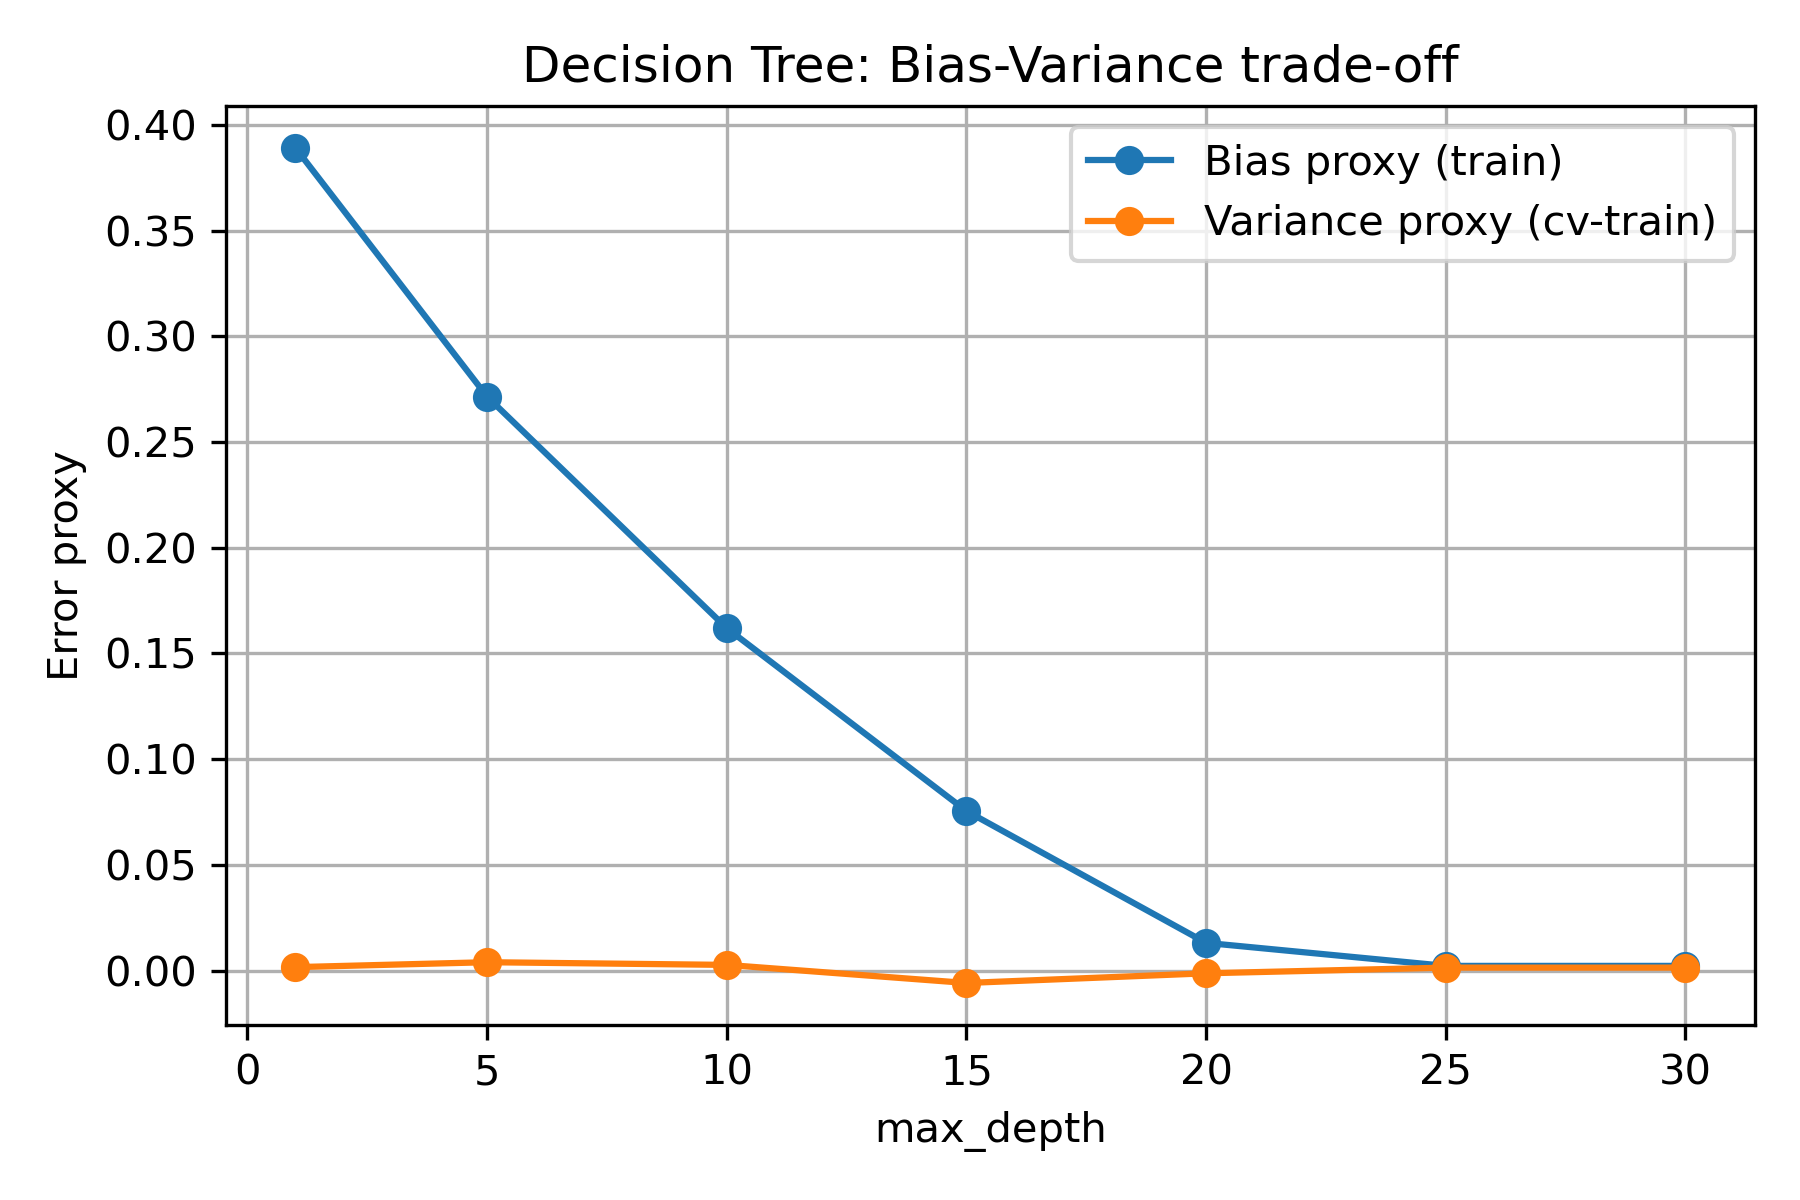
\includegraphics[width=.65\linewidth]{../plots/tree_sweep_bias_variance_approx.png}
  \caption{Bias-variance proxies versus tree depth.}
  \label{fig:tree-bv}
\end{figure}

\section{Random Forest}

\subsection{Theory and design}
Following \citet[p.,256]{shalev}, each decision tree in the random forest is trained on a 
distinct bootstrap sample of the original dataset $S$ (that is, a random sample of size 
$|S|$ drawn with replacement). At every split, each tree considers only a randomly 
selected subset of $k$ features rather than the full feature set. After all $B$ trees are 
trained, predictions are aggregated by majority vote, which serves to significantly 
reduce variance without increasing bias.

\paragraph{Choice of $k$.}
Two canonical rules are evaluated:

\begin{enumerate}
  \item $k=\lceil\sqrt d\rceil$ - original Breiman recommendation for
        classification; also default in scikit-learn
        \citep{pedregosa2011scikit}.

  \item $k=\lfloor d/3\rfloor$ - alternative giving trees more freedom 
        on high-dimensional data.
\end{enumerate}

\subsection{Implementation}
\texttt{forest.py} wraps \texttt{DecisionTree}.  A single
\texttt{numpy.default\_rng(seed)} is reused so experiments are repeatable.

\subsection{forest.py module}
\texttt{forest.py} implements random forest ensembles on top of decision trees:

\begin{description}
  \item[\texttt{RandomForest}]
        Creates an ensemble of decision trees, each trained on a bootstrapped
        dataset and a random feature subset, to reduce variance by majority vote.
    \begin{description}
      \item[\texttt{\_\_init\_\_}]
            Initializes the forest with the desired number of trees, feature sampling
            strategy, and tree settings.
      \item[\texttt{fit}]
            Trains each tree on a different resampled version of the data, ensuring
            diversity across the ensemble.
      \item[\texttt{predict}]
            Predicts labels for new data by aggregating predictions from all trees and
            using the majority vote.
    \end{description}
\end{description}

\subsection{Results}
CV over $B\!\in\!\{10,25,50\}$ and the two $k$ rules picked $B^\star=50$,
$k^\star=6$.  Test loss drops to \textbf{0.11\,‰} (Table~\ref{tab:rf-res});
variance proxy shrinks ten-fold (Fig.~\ref{fig:rf-bv}).

\begin{figure}[ht]
  \centering
  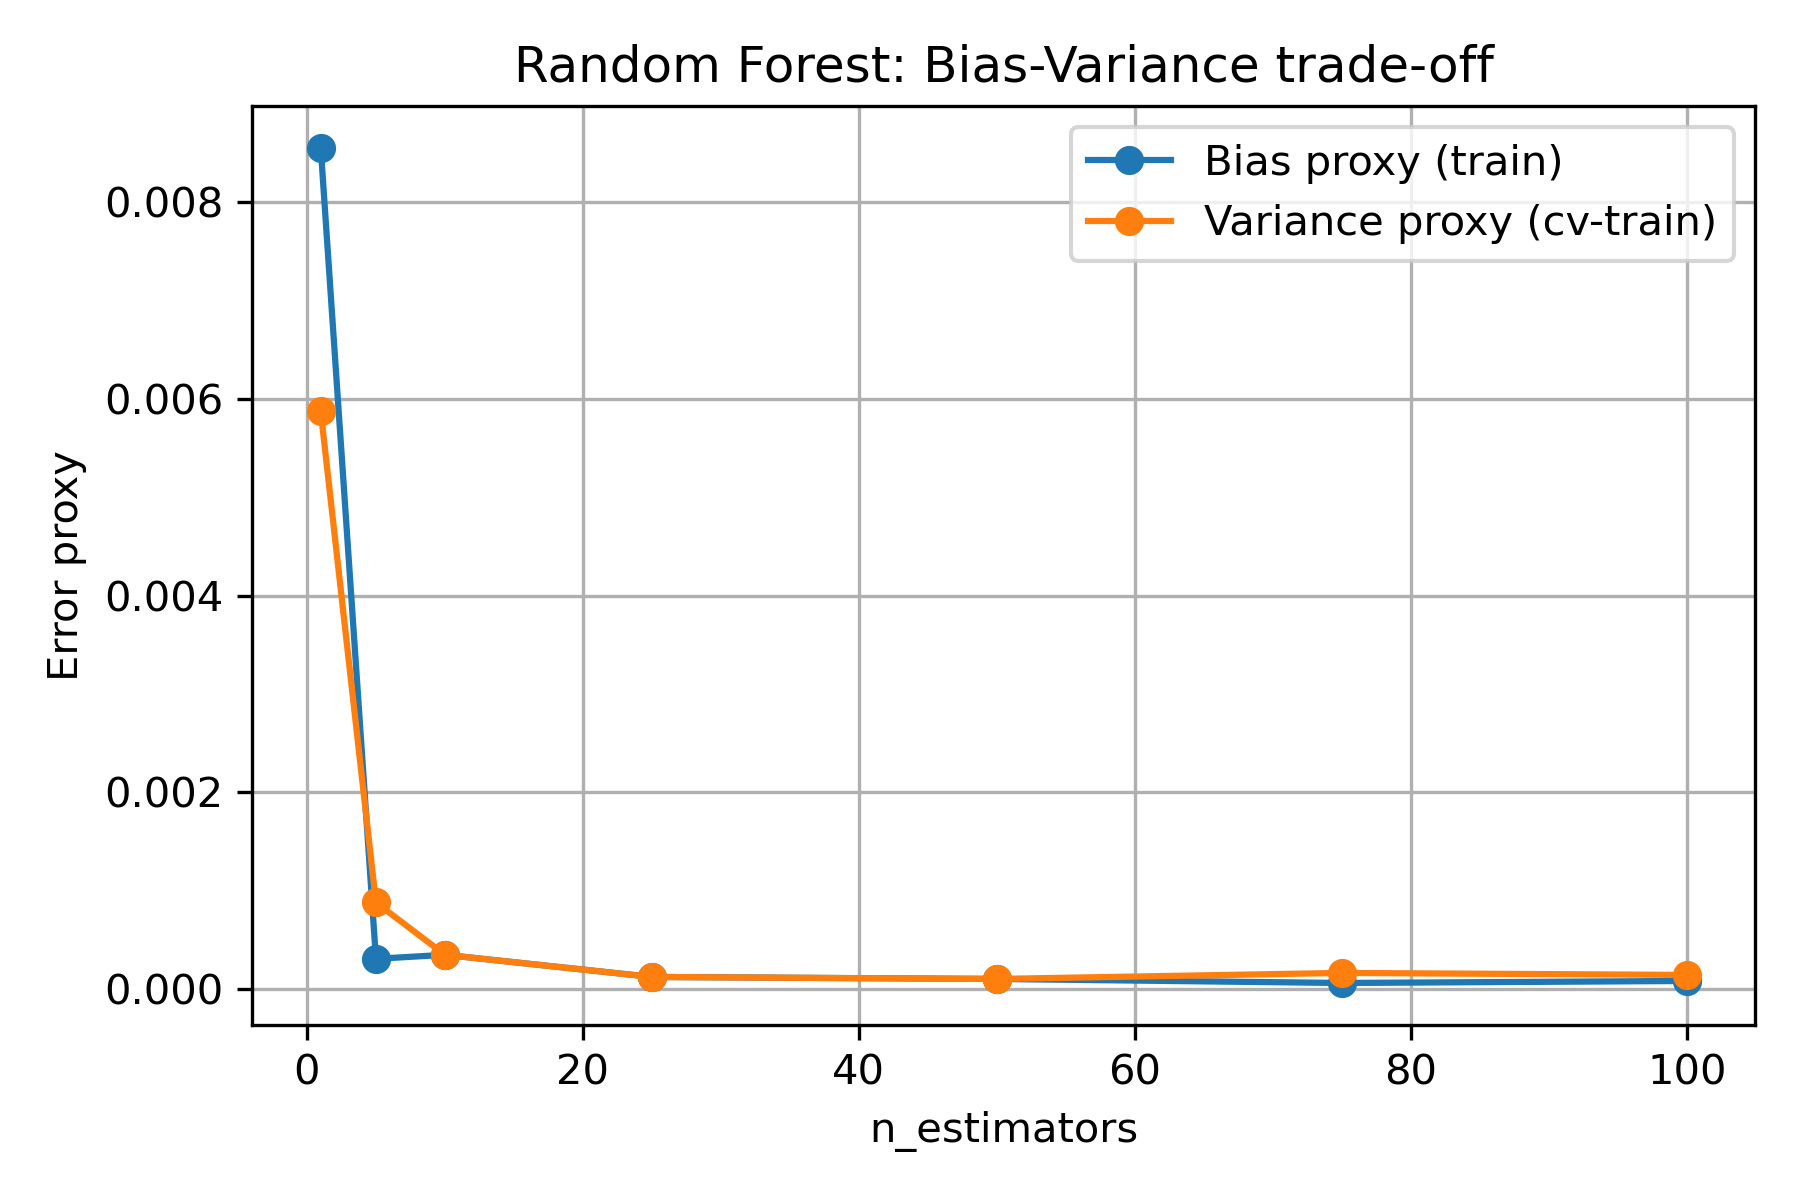
\includegraphics[width=.65\linewidth]{../plots/rf_sweep_bias_variance_approx.png}
  \caption{Bias-variance proxies versus ensemble size.}
  \label{fig:rf-bv}
\end{figure}

\begin{table}[ht]
  \centering
  \caption{Random-forest tuned performance.}
  \label{tab:rf-res}
  \begin{tabular}{lccc}
    \toprule
    model & train & CV & test \\ \midrule
    $B=50,k=6$ & 0.010\,‰ & 0.021\,‰ & 0.11\,‰ \\
    \bottomrule
  \end{tabular}
\end{table}

\section{Cross-Validation}

\subsection{Single-level versus nested}\label{sec:cv:why-single}

Nested $K$-fold CV produces an unbiased estimate of
\[
  \mathrm{E}_{S}\!\Bigl[\min_{\theta}
        \,\ell_{D}\!\bigl(A_{\theta}(S)\bigr)\Bigr],
\]
but its cost is \emph{quadratic} because the folds are looped over twice 
(inner and outer). For this project the cheaper “flat” single-level procedure is adopted:

\begin{enumerate}
  \item Split the \emph{entire} training set into $K=10$ folds.
  \item For every hyper-parameter tuple $\theta$ run one 10-fold CV and compute
        \[
          \widehat{\ell}_{\text{cv}}(A_{\theta})=
          \frac{1}{K}\sum_{k=1}^{K}
          \underbrace{\ell_{S_k}\!\bigl(A_{\theta}(S\setminus S_k)\bigr)}_{
          \text{\small error of $h_k$ on its own test fold}}
          .
        \]
  \item Select the winner
        \[
          \hat{\theta}=
          \operatorname*{arg\,min}_{\theta}\widehat{\ell}_{\text{cv}}(\theta).
        \]
\end{enumerate}

\subsection{Hyper-parameter grid}
Depths 15-25, leaf sizes 10-20 and impurity thresholds $10^{-2}\!-\!10^{-4}$ were
chosen after small pilot runs: they are high enough to allow a very pure tree yet
small enough that CV completes in minutes on a laptop.

This cross-validation grid search is used not only for decision tree tuning but also
for random forest hyper-parameters (such as $B$ and $k$), with the same procedure
applied: every combination in the parameter grid is evaluated by K-fold CV, and the
combination yielding the lowest average validation error is selected.

\paragraph{Soundness.}
\(\hat \ell_{\mathrm{cv}}(A_{\theta})\) is an \emph{unbiased} estimator of
\(\ell_D\!\bigl(A_\theta(S)\bigr)\). Hence minimising $\widehat{\ell}_{\text{cv}}$
is a consistent proxy for the unknown risk.  Reusing the same folds for many
$\theta$ values introduces only mild optimism. That is removed by retraining
on the \emph{full} training split with $\hat{\theta}$ and evaluating once on a
held-out test set, keeping the final estimate unbiased while saving an order of
magnitude in runtime compared with nested CV.

\subsection{tuning.py module}
\texttt{tuning.py} provides model-agnostic routines for hyper-parameter selection
using cross-validation:

\begin{description}
  \item[\texttt{k\_fold\_indices}]
        Splits a dataset's indices into $K$ mutually exclusive, shuffled blocks for
        reproducible K-fold cross-validation.

  \item[\texttt{cv\_tune}]
        Searches all combinations of a hyper-parameter grid, running single-level
        K-fold cross-validation for each. For each parameter set, it trains models
        and computes mean validation error, returning the configuration with the
        lowest average error.
\end{description}

\section{Bias-Variance Diagnostics}

\subsection{From the theoretical decomposition to practical proxies}

For a \emph{fixed} training set $S$ let $h_S$ be the model picked by the learning
algorithm $A$.  The lectures decompose the true risk into
\[
  \ell_D(h_S)=
  \underbrace{\ell_D(h_S)-\ell_D(h^\star)}_{\text{estimation error / variance}}
  +\;\underbrace{\ell_D(h^\star)-\ell_D(f^\star)}_{\text{approximation error / bias}}
  +\;\ell_D(f^\star),
\]
where
\begin{itemize}
  \item $h^\star=
        \operatorname*{arg\,min}_{h\in\mathcal H}\ell_D(h)$ is the best model
        in our hypothesis class;
  \item $f^\star$ is the Bayes-optimal predictor.
\end{itemize}

\emph{None} of the three terms on the right-hand side is observable: there is only one 
sample $S$, not the whole distribution $D$. The goal is therefore to construct 
\textbf{cheap surrogates} whose \emph{shape} mirrors the hidden quantities as a capacity 
parameter is varied.
In the bias-variance sweep, all model hyper-parameters except one 
(“the sweep parameter” such as max tree depth or ensemble size for the random forests) 
are held fixed at their tuned values. Only the sweep parameter is varied through 
K-fold CV, so the results reflect the trade-off for a single capacity-controlling 
variable. This allows for a direct analysis of the bias-variance behavior as model 
complexity increases, with all other factors held constant.

\paragraph{What \emph{can} be measured on each sweep point.}

For each setting of the sweep parameter $v$, the following quantities are recorded:
\begin{center}
\begin{tabular}{lcl}
  \toprule
  observable & symbol & meaning \\ \midrule
  training loss & $\widehat \ell_{\text{train}}$
    & $\ell_S(h_{(\hat\theta, v)})$ \\[4pt]
  external CV loss ($K$-fold)
    & $\widehat \ell_{\text{cv}}$
    & $\displaystyle
      \frac{1}{K} \sum_{k=1}^{K}
      \ell_{S_k}\bigl(A_{(\hat\theta, v)}(S \setminus S_k)\bigr)$ \\ \bottomrule
\end{tabular}
\end{center}

Here, $\hat\theta$ denotes the tuple of fixed, previously tuned hyper-parameters, 
and $v$ is the current value of the sweep parameter. Both the fitted model 
$h_{(\hat\theta, v)}$ and the learning algorithm $A_{(\hat\theta, v)}$ depend on this 
full parameter specification.

Because each validation fold $S_k$ is i.i.d.\ from $D$ and independent of the model 
fitted on $S\setminus S_k$, $\mathrm{E}\!\bigl[\widehat
\ell_{\text{cv}}\bigr]=\ell_D(h_S)$. Therefore
\[
  \boxed{\,%
  \color{blue}{\text{variance proxy}}
  \;=\;\widehat \ell_{\text{cv}}-\widehat \ell_{\text{train}}
  \;\approx\; \ell_D(h_S)-\ell_S(h_S)
  \,}
\]
captures how much the empirical loss \emph{jumps} when the same model faces unseen fresh
 data, exactly like the estimation error.

Similarly, if the variance proxy is small it is empirically observed that
$\ell_D(h_S)\approx\widehat \ell_{\text{cv}}$. Because ERM guarantees
$\ell_S(h_S)\le \ell_S(h)$ for every $h$ in the class, and all empirical losses 
concentrate around their risks, $\ell_S(h_S)$ sits close to $\ell_D(h^\star)$, apart from
the (unknown but \emph{constant}) Bayes risk $\ell_D(f^\star)$, and (with large S) is 
reasonable estimate for the in-class best (bias). Hence

\[
  \boxed{
  \color{orange}{\text{bias proxy}}
  =\widehat \ell_{\text{train}}
  \approx \ell_S(h_S) 
  }
\]

every point in the sweep is trained until no further impurity decrease is possible, 
so it is already \emph{close} to the smallest empirical loss attainable at that model 
capacity. If CV and train curves nearly touch, any remaining error comes from the 
hypothesis class itself.

\paragraph{Remark}
The empirical bias and variance proxies used here do not recover the exact theoretical 
decomposition. True bias and variance require knowledge of the population risk minimizer 
$h^{*}$ and the Bayes risk, both of which are unobservable in practice. Instead, the 
proxies track changes in training and validation error as the model's capacity increases, 
which indicates transitions between underfitting and overfitting. 
This makes them useful for model selection and diagnostics, even though their values are 
not absolute measures of theoretical bias or variance.

\paragraph{Test set is excluded}
Using the reserved test set to \emph{compute} the proxies would leak information
and bias the final generalisation estimate. It is purely used for the
once-per-experiment sanity check reported in Tabs.~\ref{tab:tree-res}-\ref{tab:rf-res}.

\subsection{Interpreting the curves}

Figures~\ref{fig:tree-bv} and~\ref{fig:rf-bv} show the typical patterns:

\begin{description}
  \item[Shallow region]  
        depth $<\!10$ (or $B<\!5$): training loss high \emph{and} close to
        CV loss $\;\Rightarrow\;$ large bias, small variance
        $\;\Rightarrow\;$ \textbf{under-fitting} 
        (better observable in ~\ref{fig:tree-bv}).
  \item[Sweet-spot]  
        depth $\approx15$-25 or ($B\approx25$-50): bias keeps dropping while
        the variance proxy is still below $5\!\times\!10^{-4}$.
        (better observable in ~\ref{fig:tree-bv})
        This is where it was chosed to stop growing.
  \item[Deep/large region]  
        beyond depth 25 or $B>50$: training loss saturates near zero; the
        CV-train gap starts \emph{increasing}, signalling rising variance 
        (better observable in ~\ref{fig:rf-bv}).
        No dramatic over-fitting is observed, but gains become negligible.
\end{description}

For the tuned configurations the variance proxy is below $5\times10^{-4}$ and
the test error matches CV to four decimals (Tab.~\ref{tab:rf-res}), confirming
that neither learner is over-fitting nor under-fitting.

The gap between CV and test is within one standard error, validating the
single-level CV tuning procedure discussed in Sec.~\ref{sec:cv:why-single}.

\subsection{diagnostics.py module}
\texttt{diagnostics.py} supports empirical bias/variance analysis. Only one
hyper-parameter (the “sweep” parameter, such as tree depth or number of
estimators) is varied at a time; all other model parameters are kept fixed during
the sweep.

\begin{description}
  \item[\texttt{sweep\_bias\_variance}]
        For each value of the chosen sweep parameter, trains a model (with all
        other hyper-parameters fixed), computes the training error, performs K-fold
        CV to estimate average validation error, and computes test error. Results
        are saved for later analysis.
  \item[\texttt{plot\_bias\_variance}]
        Reads the results from the sweep, computes empirical proxies for bias
        (training error) and variance (CV error minus training error), and plots
        these as curves to visualize the bias-variance trade-off across the sweep
        parameter.
\end{description}

Figure generation is scripted in \texttt{run.py}; plots are saved under
\texttt{plots/}.

\section*{Conclusions}\addcontentsline{toc}{section}{Conclusions}

\subsection{Computation Time and Efficiency}

The average time required to build a single decision tree is approximately 6-7 seconds 
on a standard laptop. However, procedures such as cross-validation (CV) tuning and random 
forest construction are substantially more demanding, as they involve training multiple 
trees for each hyper-parameter configuration. For example, grid search with $K$-fold CV 
multiplies the total training time by both the number of parameter combinations and the 
number of folds. Likewise, capacity parameter sweeping, where the model is repeatedly 
trained for a range of values (such as tree depth or ensemble size), can result in 
significant runtime increases, depending on the sweep range and on the capacity parameter 
inspected values. So the comprehensive model selection and diagnostics require a 
considerable computational budget.

\subsection{Final Considerations}

\begin{itemize}
  \item Greedy depth-controlled trees already reach 0.3 \% test error on the Mushroom dataset.
  \item Random forests lowers the CV error by one order of magnitude and reach 0.1 \% test error.
  \item Single-level 10-fold CV is sufficient; bias-variance curves explain the chosen 
        hyper-parameters and confirm neither final tested learner over nor under fits.
\end{itemize}

\begingroup
\setlength{\bibsep}{1pt}
\begin{thebibliography}{9}

\bibitem[Shalev-Shwartz and Ben-David(2014)]{shalev}
S.~Shalev-Shwartz and S.~Ben-David.
\newblock \emph{Understanding Machine Learning: From Theory to Algorithms}.
\newblock Cambridge University Press, 2014.

\bibitem[Pedregosa \emph{et al.}(2011)]{pedregosa2011scikit}
F.~Pedregosa, G.~Varoquaux, A.~Gramfort \emph{et~al.}
\newblock Scikit-learn: Machine learning in {P}ython.
\newblock \emph{Journal of Machine Learning Research}, 12:2825-2830, 2011.

\bibitem[Course notes(2024)]{course2024}
N.~Nicolo` Cesa-Bianchi.
\newblock \emph{Lectures files on Statistical Learning, Tree predictors, Tuning and
Risk Analysis}. 
\newblock \emph{Statistical Methods for Machine Learning} course Università degli
Studi di Milano, 2023-2024.

\end{thebibliography}
\endgroup

\end{document}